\documentclass[11pt,reqno]{amsart}

\usepackage[utf8]{inputenc}
\usepackage[T1]{fontenc}
\usepackage{amsmath,amssymb,amsfonts,amsthm,mathtools}
\usepackage{geometry}
\geometry{a4paper, top=2.5cm, bottom=2.5cm, left=2.5cm, right=2.5cm}
\usepackage{booktabs}
\usepackage{array}
\newcolumntype{L}[1]{>{\raggedright\arraybackslash}p{#1}}
\usepackage{graphicx}
\usepackage{microtype}
\usepackage{xcolor}
\usepackage{tikz}
\usetikzlibrary{shapes,arrows,positioning,calc,decorations.pathmorphing,backgrounds,fit}
\usepackage[most]{tcolorbox}
\usepackage{hyperref}

\definecolor{navyblue}{RGB}{16, 44, 87}
\definecolor{forestgreen}{RGB}{24, 92, 55}
\definecolor{burgundy}{RGB}{128, 20, 36}
\definecolor{boxbg}{RGB}{249, 250, 253}
\definecolor{boxframe}{RGB}{195, 205, 225}

\hypersetup{
    colorlinks=true,
    linkcolor=navyblue,
    citecolor=forestgreen,
    urlcolor=burgundy,
    pdftitle={An S3-Circulant Parametrization of Fermion Masses and Mixing and a Simplicial Vacuum-Energy Ansatz: Relations, Fits, and Parameter Count},
    pdfauthor={Reinaldo M. Silva-Filho}
}

% Styled theorem boxes
\tcolorboxenvironment{theorem}{
    enhanced,
    boxrule=1pt,
    colback=boxbg,
    colframe=navyblue,
    arc=3pt,
    left=8pt, right=8pt, top=6pt, bottom=6pt
}
\tcolorboxenvironment{proposition}{
    enhanced,
    boxrule=0.8pt,
    colback=boxbg,
    colframe=boxframe,
    arc=2pt,
    left=8pt, right=8pt, top=6pt, bottom=6pt
}
\tcolorboxenvironment{definition}{
    enhanced,
    boxrule=0.8pt,
    colback=white,
    colframe=forestgreen!85!black,
    arc=2pt,
    left=8pt, right=8pt, top=6pt, bottom=6pt
}

% Theorem Environments
\newtheorem{theorem}{Theorem}[section]
\newtheorem{lemma}[theorem]{Lemma}
\newtheorem{proposition}[theorem]{Proposition}
\newtheorem{corollary}[theorem]{Corollary}
\theoremstyle{definition}
\newtheorem{definition}[theorem]{Definition}
\newtheorem{example}[theorem]{Example}
\newtheorem{remark}[theorem]{Remark}

% Mathematical Macros
\newcommand{\R}{\mathbb{R}}
\newcommand{\C}{\mathbb{C}}
\newcommand{\N}{\mathbb{N}}
\newcommand{\Z}{\mathbb{Z}}
\newcommand{\Tr}{\operatorname{Tr}}
\newcommand{\diag}{\operatorname{diag}}
\newcommand{\SU}{\mathrm{SU}}
\newcommand{\SO}{\mathrm{SO}}
\newcommand{\U}{\mathrm{U}}
\newcommand{\CKM}{\mathrm{CKM}}
\newcommand{\PMNS}{\mathrm{PMNS}}
\newcommand{\circm}{\mathrm{circ}}
\newcommand{\EW}{\mathrm{EW}}
\newcommand{\Pl}{\mathrm{Planck}}
\newcommand{\GUT}{\mathrm{GUT}}

\title[$S_3$-Circulant Flavor Parametrization: Relations, Fits, Parameter Count]{An $S_3$-Circulant Parametrization of Fermion Masses\\ and Mixing and a Simplicial Vacuum-Energy Ansatz:\\ Relations, Fits, and Parameter Count}

\author{Reinaldo M. Silva-Filho}
\address{Programa de P\'os-Gradua\c{c}\~ao em Estat\'istica e Experimenta\c{c}\~ao Agropecu\'aria (PPGEE/DES)\\
Departamento de Estat\'istica (DES), Universidade Federal de Lavras (UFLA)\\
Lavras, Minas Gerais, Brazil}
\email{reinaldo.filho1@estudante.ufla.br}

\thanks{This research was supported by the Coordena\c{c}\~ao de Aperfei\c{c}oamento de Pessoal de N\'ivel Superior (CAPES) -- Finance Code 001.}

\date{\today}

% Custom title, author, and section typography
\makeatletter
\def\@settitle{\begin{center}%
  \baselineskip20\p@\relax
  \bfseries\LARGE\color{navyblue}%
  \@title
  \end{center}%
}
\def\@setauthors{%
  \begingroup
  \trivlist
  \centering\large \@topsep16\p@\relax
  \advance\hsize by-\leftmargin
  \item\relax
  \author@andify\authors
  \def\\{\protect\linebreak}%
  {\large\bfseries\color{black!85}\authors}%
  \endtrivlist
  \endgroup
}
\def\@setaddresses{\par
  \nobreak \begingroup
  \footnotesize
  \def\author##1{\par\smallskip\noindent}%
  \def\\{\check@mathfonts\cr}%
  \centering
  \addresses
  \endgroup
}
\makeatother

\begin{document}

\begin{abstract}
We study a phenomenological parametrization of flavor observables built on the permutation symmetry $S_3$ of a generation simplex $\Delta_2$, together with an ansatz for the vacuum energy on the 4-simplex $\Delta_4$. Every numerical statement is classified as an identity, a known empirical relation, a fit, or a prediction, and the continuous inputs are counted against the observables they are compared with. All numbers use PDG~2024 inputs and are reproduced by an accompanying script.
(i) Writing the charged-lepton root masses as $\sqrt{m_j} = a + 2b\cos(\delta + 2\pi j/3)$, the Koide ratio equals $Q_l = \frac13 + \frac{2b^2}{3a^2}$ for every $(a,b,\delta)$. Hence $Q_l = 2/3$ is equivalent to $b/a = 1/\sqrt2$, i.e.\ to a $45^\circ$ angle between $(\sqrt{m_e},\sqrt{m_\mu},\sqrt{m_\tau})$ and $(1,1,1)$: a reformulation of Koide's relation, which the $S_3$ structure accommodates but does not fix. Assuming it, $m_e$ and $m_\mu$ give $m_\tau = 1776.97\text{ MeV}$, $0.4\sigma$ from the measured $1776.93 \pm 0.09\text{ MeV}$.
(ii) For $(c,b,t)$ the analogous ratio is scheme dependent ($0.72$ with $\overline{\mathrm{MS}}$ masses at $M_Z$, $0.65$ with pole masses); the expression $\frac23(1+\alpha_s/\sqrt3) = 0.712$ lies in this range but has no derivation.
(iii) The Gatto--Sartori--Tonin relation $\sqrt{m_d/m_s} = 0.2242 \pm 0.0019$ agrees with $|V_{us}| = 0.2243$. The phase ansatz $\delta = \pi/3 + \alpha_s/\sqrt3 = 63.9^\circ$ lies $1.2\sigma$ below the global fit, and the Jarlskog invariant evaluated with it inherits its size from the empirical inputs $s_{23}$ and $s_{13}$. We have no geometric expression for $J_{\mathrm{CP}}$.
(iv) The dimension-five scaling $v^2/M$ with $M = 2\times10^{15}\text{ GeV}$ gives $30\text{ meV}$, the order of $\sqrt{\Delta m^2_{31}} = 50\text{ meV}$. The tri-bimaximal-Cabibbo ansatz gives $\sin^2\theta_{12} = 1/3$ ($2.0\sigma$), $\sin^2\theta_{23} = 1/2$ ($2.8\sigma$) and $\sin\theta_{13} = 0.159$--$0.160$, $4.5$--$5\sigma$ above the measured $0.148$.
(v) The face numbers of $\Delta_4$ satisfy $\chi = 1$ and $\tilde\chi = 0$, but zero-point energy is not shown to be such an alternating sum. The ansatz $\rho = M_P^4 \exp(-2\pi/(\alpha\,\mathcal{E}_\infty))$ with $\mathcal{E}_\infty = \ln 2 - \frac12$ reproduces the observed $\rho_\Lambda = (2.24\text{ meV})^4$ only for $\alpha = 0.1149$; a $1\%$ change of $\alpha$ changes $\rho$ by a factor $17$, so this is a one-parameter fit.
Nine continuous inputs (four free, five measured) and at least eight discrete choices face twelve observables. The tests that pass are the known Koide and Gatto--Sartori--Tonin relations, and the one sharp new relation, for $\theta_{13}$, disagrees with the data.
\end{abstract}

\maketitle

\tableofcontents

\newpage

% ==============================================================================
\section{Introduction}
% ==============================================================================

Two parameter problems motivate this paper:
\begin{enumerate}
    \item \textbf{Flavor.} With massless neutrinos the Standard Model has thirteen flavor parameters: nine charged-fermion masses, three CKM angles and one CKM phase. Neutrino masses and mixing add at least seven more (three masses, three angles, one Dirac phase), and two Majorana phases if neutrinos are Majorana. The masses range from $m_e = 0.511\text{ MeV}$ to $m_t \approx 173\text{ GeV}$, and the Standard Model does not explain their values \cite{weinberg1967model,kobayashi1973cp,pdg2024}.
    \item \textbf{Vacuum energy.} A zero-point energy density cut off at the Planck scale is of order $M_P^4$, i.e.\ $3.5\times10^{73}\text{ GeV}^4$ for the reduced Planck mass and $2.2\times10^{76}\text{ GeV}^4$ for $M_P = G_N^{-1/2}$, while the observed dark-energy density is $\rho_\Lambda = 2.5\times10^{-47}\text{ GeV}^4$ \cite{weinberg1989cosmological,planck2018}: a ratio of order $10^{-121}$ to $10^{-123}$.
\end{enumerate}

This paper does not solve either problem. It collects a set of relations suggested by the permutation symmetry of a generation simplex $\Delta_2$ and by the combinatorics of the 4-simplex $\Delta_4$, and it examines each of them with PDG~2024 inputs \cite{pdg2024}. Each numerical statement is placed in one of four classes:
\begin{itemize}
    \item \emph{identity}: true by algebra, with no empirical content;
    \item \emph{known relation}: an empirical relation published earlier (Koide, Gatto--Sartori--Tonin, tri-bimaximal mixing), restated in the present language;
    \item \emph{fit}: a formula with at least one input chosen to reproduce the observable it is compared with;
    \item \emph{prediction}: a number obtained from inputs that do not include the observable, and that could have failed.
\end{itemize}
Section~\ref{sec:count} counts continuous inputs against observables. The material overlaps with the phenomenological section of the author's monograph \cite[Ch.~12, Sec.~7]{silvafilho2026book}, and the conventions here follow it. All numbers are recomputed by the script \texttt{verify\_fermion\_paper\_numbers.py} in the paper's folder, which uses independent oracles and negative controls.

\begin{figure}[htbp]
\centering
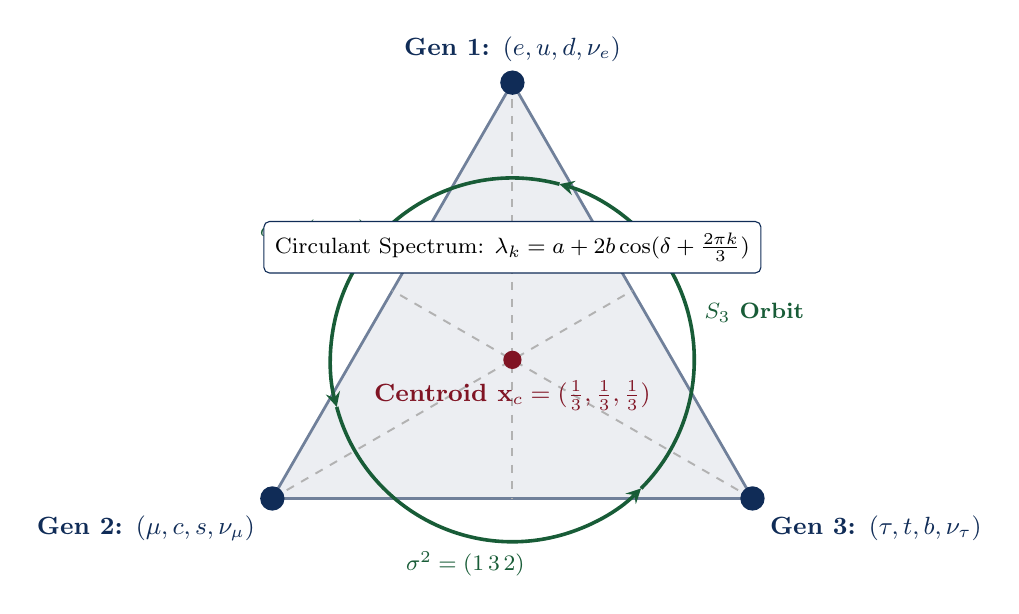
\begin{tikzpicture}[scale=1.1, >=stealth]
    % Flavor triangle Delta_2
    \coordinate (v1) at (90:3.2);
    \coordinate (v2) at (210:3.2);
    \coordinate (v3) at (330:3.2);
    \coordinate (c) at (0,0);

    % Shaded face
    \fill[navyblue!8, draw=navyblue!60, line width=1pt] (v1) -- (v2) -- (v3) -- cycle;

    % Medians and Barycenter
    \draw[dashed, gray!60, line width=0.7pt] (v1) -- ($(v2)!0.5!(v3)$);
    \draw[dashed, gray!60, line width=0.7pt] (v2) -- ($(v1)!0.5!(v3)$);
    \draw[dashed, gray!60, line width=0.7pt] (v3) -- ($(v1)!0.5!(v2)$);

    % Centroid
    \fill[burgundy] (c) circle (3pt) node[below=4pt, font=\small\bfseries, color=burgundy] {Centroid $\mathbf{x}_c = (\frac{1}{3}, \frac{1}{3}, \frac{1}{3})$};

    % Vertices (generations)
    \fill[navyblue] (v1) circle (4pt) node[above=4pt, font=\bfseries\small] {Gen 1: $(e, u, d, \nu_e)$};
    \fill[navyblue] (v2) circle (4pt) node[below left=4pt, font=\bfseries\small] {Gen 2: $(\mu, c, s, \nu_\mu)$};
    \fill[navyblue] (v3) circle (4pt) node[below right=4pt, font=\bfseries\small] {Gen 3: $(\tau, t, b, \nu_\tau)$};

    % Permutation arrows S3
    \draw[->, line width=1.3pt, forestgreen] (75:2.1) arc (75:195:2.1) node[midway, left=2pt, font=\footnotesize\bfseries] {$\sigma = (1\,2\,3)$};
    \draw[->, line width=1.3pt, forestgreen] (195:2.1) arc (195:315:2.1) node[midway, below=2pt, font=\footnotesize\bfseries] {$\sigma^2 = (1\,3\,2)$};
    \draw[->, line width=1.3pt, forestgreen] (315:2.1) arc (315:435:2.1) node[midway, right=2pt, font=\footnotesize\bfseries] {$S_3$ Orbit};

    % Label
    \node[draw=navyblue, fill=white, rounded corners=2pt, inner sep=4pt, font=\footnotesize] at (0, 1.3) {Circulant Spectrum: $\lambda_k = a + 2b \cos(\delta + \frac{2\pi k}{3})$};
\end{tikzpicture}
\caption{The generation simplex $\Delta_2$ with its $S_3$ action. A Hermitian circulant matrix on the three vertices has eigenvalues $\lambda_k = a + 2b\cos(\delta + 2\pi k/3)$; its eigenvectors do not depend on $(a,b,\delta)$ (Remark~\ref{rem:dft}).}
\label{fig:flavor_simplex}
\end{figure}

% ==============================================================================
\section{The Generation Simplex \texorpdfstring{$\Delta_2$}{Delta 2} and the Circulant Ansatz}
% ==============================================================================

\subsection{The Generation Simplex}
Let $\Delta_2 = \{(x_1, x_2, x_3) \in \mathbb{R}_{\ge 0}^3 : x_1 + x_2 + x_3 = 1\}$, with one vertex per generation. The permutation representation of $S_3$ on $\R^3$ decomposes into irreducible components as
\begin{equation}
    V_{\mathrm{flavor}} \cong \mathbf{1} \oplus \mathbf{2}.
\end{equation}
The number of generations is an input: choosing $\Delta_2$ fixes it at three, and the analogous decomposition $\R^n \cong \mathbf{1} \oplus (\mathbf{n-1})$ holds for every $n$.

\subsection{Circulant Ansatz}
Gauge invariance under $\SU(3)_c \times \SU(2)_L \times \U(1)_Y$ allows an arbitrary complex $3\times3$ Yukawa matrix in each charged sector. We \emph{assume} that the matrix $\mathbf{C}$ whose eigenvalues are the root masses $\sqrt{m_k}$ is a Hermitian circulant, i.e.\ commutes with the cyclic permutation $\sigma = (1\,2\,3)$:
\begin{equation}\label{eq:circulant_Y}
    \mathbf{C}(a, b, \delta) \coloneqq \begin{pmatrix}
        a & b e^{i\delta} & b e^{-i\delta} \\
        b e^{-i\delta} & a & b e^{i\delta} \\
        b e^{i\delta} & b e^{-i\delta} & a
    \end{pmatrix}, \quad a, b \ge 0, \; \delta \in [0, 2\pi).
\end{equation}
Its eigenvalues are $\lambda_k = a + 2b \cos\left( \delta + \frac{2\pi k}{3} \right)$, $k \in \{0, 1, 2\}$. The mass matrix is $\mathbf{M} = \mathbf{C}^2$, again a Hermitian circulant, with eigenvalues $\lambda_k^2 = m_k$; in the notation of \cite[Ch.~12, Sec.~7]{silvafilho2026book} this is $\mathbf{M} = \frac{v}{\sqrt2}\mathbf{Y}_{\mathrm{circ}}$ with $\mathbf{Y}_{\mathrm{circ}} = \frac{\sqrt2}{v}\mathbf{C}^2$ and $v = (\sqrt2\,G_F)^{-1/2} = 246.22\text{ GeV}$.

For the product geometry $\Delta_4 \times \Delta_2$ the mass matrix enters through the Dirac operator of a product of spectral triples \cite{chamseddine2007gravity},
\begin{equation}\label{eq:dirac_product}
    \boldsymbol{\mathcal{D}} = \boldsymbol{\mathcal{D}}_{\Delta_4} \otimes \mathbf{1} + \gamma_5 \otimes \mathbf{M}.
\end{equation}
Since $\gamma_5$ anticommutes with $\boldsymbol{\mathcal{D}}_{\Delta_4}$, $\boldsymbol{\mathcal{D}}^2 = \boldsymbol{\mathcal{D}}_{\Delta_4}^2 \otimes \mathbf{1} + \mathbf{1} \otimes \mathbf{M}^2$, and a mode of momentum $k$ in a generation of mass $m$ has eigenvalues $\pm\sqrt{k^2 + m^2}$. With $\mathbf{1}$ in place of $\gamma_5$ the eigenvalues would be $\pm|k| + m$, without a gap. As in \cite[Ch.~12, Sec.~7]{silvafilho2026book}, boundary conditions on the simplex $\Delta_4$ are not specified, and \eqref{eq:dirac_product} is used only for its algebraic structure.

\begin{remark}\label{rem:dft}
Every circulant matrix is diagonalized by the discrete Fourier matrix $F_{jk} = \omega^{jk}/\sqrt3$, $\omega = e^{2\pi i/3}$, independently of $(a,b,\delta)$. If the up-type and the down-type mass matrices are both circulant in the same basis, they are diagonalized by the same unitary, and the CKM matrix is a permutation matrix up to phases. The circulant ansatz therefore does not produce the Cabibbo angle. The mixing relations of Sections~\ref{sec:cabibbo}--\ref{sec:cp} are stated separately and do not follow from \eqref{eq:circulant_Y}.
\end{remark}

% ==============================================================================
\section{Charged Leptons: the Koide Relation in Circulant Form}
% ==============================================================================

\begin{proposition}[Koide ratio of a circulant spectrum]\label{thm:koide_exact}
Let $\mathbf{v} = (v_0, v_1, v_2)$ with $v_j = a + 2b\cos(\delta + 2\pi j/3)$, $a, b \ge 0$, and write $\mathbf{v} = \mathbf{v}_{\mathbf{1}} + \mathbf{v}_{\mathbf{2}}$ with $\mathbf{v}_{\mathbf{1}} = a(1,1,1)$ in the trivial representation and $\mathbf{v}_{\mathbf{2}}$ in the trace-zero plane. Then $\|\mathbf{v}_{\mathbf{1}}\|^2 = 3a^2$, $\|\mathbf{v}_{\mathbf{2}}\|^2 = 6b^2$ and
\begin{equation}\label{eq:koide_general}
    Q \coloneqq \frac{\sum_j v_j^2}{\left(\sum_j v_j\right)^2} = \frac13 + \frac{2b^2}{3a^2}.
\end{equation}
Consequently
\begin{equation}\label{eq:norm_equipartition}
    Q = \frac23 \iff \|\mathbf{v}_{\mathbf{2}}\|^2 = \|\mathbf{v}_{\mathbf{1}}\|^2 \iff \frac{b}{a} = \frac{1}{\sqrt2} \iff \angle\big(\mathbf{v}, (1,1,1)\big) = 45^\circ.
\end{equation}
\end{proposition}

\begin{proof}
$\sum_j \cos(\delta + 2\pi j/3) = 0$ and $\sum_j \cos^2(\delta + 2\pi j/3) = \frac32$, so $\sum_j v_j = 3a$ and $\sum_j v_j^2 = 3a^2 + 6b^2$. The angle $\theta$ between $\mathbf{v}$ and $(1,1,1)$ satisfies $\cos^2\theta = (\sum_j v_j)^2/(3\sum_j v_j^2) = 1/(3Q)$.
\end{proof}

\begin{remark}[Status]
Proposition~\ref{thm:koide_exact} is an identity. Every value $Q \in [\frac13, 1]$ is attained by a circulant spectrum with nonnegative entries, so the $S_3$ structure accommodates $Q = 2/3$ but does not select it; the condition $b/a = 1/\sqrt2$ is the Koide relation \cite{koide1982,koide1983fermion} in another form, as noted in \cite[Ch.~12, Sec.~7]{silvafilho2026book}. Applied to $v_j = \sqrt{m_j}$, the model has three parameters $(a, b, \delta)$ for three masses; imposing $b/a = 1/\sqrt2$ leaves two, fixed by $m_e$ and $m_\mu$.
\end{remark}

\textbf{Prediction.} With $m_e = 0.51099895\text{ MeV}$ and $m_\mu = 105.6583755\text{ MeV}$ \cite{pdg2024}, $Q = 2/3$ gives
\begin{equation}
    m_\tau = 1776.969\text{ MeV},
\end{equation}
$0.43\sigma$ above the PDG~2024 value $m_\tau = 1776.93 \pm 0.09\text{ MeV}$. This is the prediction of \cite{koide1982,koide1983fermion}. Conversely, the measured masses give $Q_l = 0.6666645 \pm 0.0000051$ (uncertainty from $m_\tau$), and the angle in \eqref{eq:norm_equipartition} is $44.9999^\circ$.

% ==============================================================================
\section{Quarks: a Scheme-Dependent Ratio}\label{sec:quark}
% ==============================================================================

For quarks the masses are not physical observables in the same sense as for leptons: they depend on the renormalization scheme and scale. For the heavy triplet $(c, b, t)$,
\begin{equation}
    Q_{cbt} \coloneqq \frac{m_c + m_b + m_t}{\left(\sqrt{m_c} + \sqrt{m_b} + \sqrt{m_t}\right)^2}
    = \begin{cases}
        0.720 & \overline{\mathrm{MS}} \text{ masses at } \mu = M_Z,\\
        0.648 & \text{pole masses},
    \end{cases}
\end{equation}
with $(m_c, m_b, m_t) = (0.620, 2.839, 168.26)\text{ GeV}$ at $M_Z$ \cite{huang2021precise} and pole masses $(1.67, 4.78, 172.57)\text{ GeV}$ \cite{pdg2024}. Our own two-loop running from the PDG~2024 values $m_c(m_c)$, $m_b(m_b)$, $m_t(m_t)$ gives $0.718$. Other triplets give different values, e.g.\ $Q_{dsb} = 0.73$ and $Q_{uct} = 0.85$.

\begin{remark}
The expression $\frac23\left(1 + \alpha_s(M_Z)/\sqrt3\right) = 0.7121$ lies in the range $[0.65, 0.72]$ spanned by the two schemes. It is a numerical fit with $\alpha_s(M_Z)$ as input and no derivation: the factor $1/\sqrt3$ is neither the color Casimir $C_F = 4/3$ nor a known one-loop coefficient (the form $\frac23(1 + C_F\alpha_s/\pi)$ gives $0.700$). Given the spread between schemes, agreement with it carries no evidential weight \cite[Ch.~12, Sec.~7]{silvafilho2026book}.
\end{remark}

% ==============================================================================
\section{The Cabibbo Angle: the Gatto--Sartori--Tonin Relation}\label{sec:cabibbo}
% ==============================================================================

The Gatto--Sartori--Tonin relation \cite{cabibbo1963unitary,gatto1968relation} is the known empirical relation $\sin\theta_C \approx \sqrt{m_d/m_s}$. With the PDG~2024 $\overline{\mathrm{MS}}$ masses at $2\text{ GeV}$, $m_d = 4.70 \pm 0.07\text{ MeV}$ and $m_s = 93.5 \pm 0.8\text{ MeV}$ (the ratio is scale independent in QCD),
\begin{equation}
    \sqrt{\frac{m_d}{m_s}} = 0.2242 \pm 0.0019, \qquad |V_{us}| = 0.22431 \pm 0.00085 \ \text{\cite{pdg2024}},
\end{equation}
an agreement at the $0.05\%$ level, well inside the $0.9\%$ uncertainty of the mass ratio.

\begin{remark}
The factor $(1 + \alpha_s/(4\pi))$ changes the left side by $0.94\%$, to $0.2263$. It has no derivation here, and its size is comparable to the input uncertainty, so it can be neither confirmed nor excluded. Neither the relation nor the factor follows from the geometry of $\Delta_2$: by Remark~\ref{rem:dft}, the circulant ansatz alone gives no Cabibbo mixing. Below, the relation is used with the measured $m_d/m_s$ as an input.
\end{remark}

% ==============================================================================
\section{Neutrinos: Mass Scale and a Tri-Bimaximal-Cabibbo Ansatz}\label{sec:neutrino}
% ==============================================================================

\textbf{Mass scale.} The dimension-five operator $(LH)(LH)/M$ \cite{weinberg1979baryon}, generated for instance by a type-I seesaw with Dirac mass of order $v$, gives
\begin{equation}
    m_\nu \sim \frac{v^2}{M} = \frac{(246.22\text{ GeV})^2}{2.0 \times 10^{15}\text{ GeV}} = 30.3\text{ meV}.
\end{equation}
Dimensions: $[v^2/M] = \text{GeV}^2/\text{GeV} = \text{GeV}$. In normal ordering with $m_1 \approx 0$ the heaviest mass is
\begin{equation}
    m_3 \approx \sqrt{\Delta m^2_{32} + \Delta m^2_{21}} = 50.3\text{ meV} \ \text{\cite{pdg2024}},
\end{equation}
so the orders of magnitude agree. The scale $M$ is a free parameter, and $M = 1.2\times10^{15}\text{ GeV}$ reproduces $m_3$. The normalization is convention dependent: with $v/\sqrt2$ in place of $v$ the estimate is $15.2\text{ meV}$. This is a one-parameter order-of-magnitude estimate, not a prediction. The simplicial trace operators of \cite[Ch.~5]{silvafilho2026book} do not produce it.

\textbf{Mixing.} Tri-bimaximal mixing \cite{harrison2002tribimaximal} combined with $\sin\theta_{13} = \sin\theta_C/\sqrt2$ \cite{king2012tbc} gives
\begin{equation}
    \sin^2 \theta_{12} = \frac{1}{3}, \quad \sin^2 \theta_{23} = \frac{1}{2}, \quad \sin \theta_{13} = \frac{\sin \theta_C}{\sqrt{2}} = 0.159\text{--}0.160,
\end{equation}
where the range corresponds to $\sin\theta_C = |V_{us}|$ or $0.2263$. The PDG~2024 values (normal ordering) are $\sin^2\theta_{12} = 0.307 \pm 0.013$, $\sin^2\theta_{23} = 0.558^{+0.015}_{-0.021}$ and $\sin^2\theta_{13} = (2.19 \pm 0.07)\times10^{-2}$, i.e.\ $\sin\theta_{13} = 0.1480 \pm 0.0024$ \cite{maki1962remarks,pdg2024}. The pulls are $+2.0\sigma$, $-2.8\sigma$ and $+4.5\sigma$ to $+5.1\sigma$ respectively. These are known ansätze with no free continuous parameter; the relation for $\theta_{13}$ is disfavored by the data. The phrase \emph{isotropic delocalization on $\Delta_2$} describes the trimaximal column $(1,1,1)/\sqrt3$ of the tri-bimaximal matrix; it does not derive the other two columns.

% ==============================================================================
\section{CP Violation: a Phase Ansatz and the Jarlskog Invariant}\label{sec:cp}
% ==============================================================================

Consider the ansatz
\begin{equation}\label{eq:delta_ansatz}
    \delta = \frac{\pi}{3} + \frac{\alpha_s(M_Z)}{\sqrt{3}} = 1.1153\text{ rad} = 63.90^\circ
\end{equation}
for the phase of the standard parametrization of the CKM matrix. Neither the offset $\pi/3$ nor the term $\alpha_s/\sqrt3$, the same factor as in Section~\ref{sec:quark}, is derived; the circulant phase $\delta$ of \eqref{eq:circulant_Y} does not enter the CKM matrix (Remark~\ref{rem:dft}). The PDG~2024 global fit gives $\delta = 1.147 \pm 0.026\text{ rad} = (65.7 \pm 1.5)^\circ$ \cite{pdg2024}, a pull of $-1.2\sigma$.

The Jarlskog invariant \cite{jarlskog1985commutator}, $J_{\mathrm{CP}} = \operatorname{Im}(V_{us}V_{cb}V_{ub}^*V_{cs}^*)$, is dimensionless and independent of the parametrization; in the standard parametrization
\begin{equation}
    J_{\mathrm{CP}} = c_{12} c_{23} c_{13}^2 \, s_{12} s_{23} s_{13} \sin\delta.
\end{equation}
With $s_{12} = 0.2263$ (Section~\ref{sec:cabibbo}), $\delta$ from \eqref{eq:delta_ansatz}, and the fitted $s_{23} = 0.04183$ and $s_{13} = 0.003732$ \cite{pdg2024},
\begin{equation}
    J_{\mathrm{CP}} = 3.09 \times 10^{-5}, \qquad J_{\mathrm{CP}}^{\mathrm{fit}} = \left(3.12^{+0.13}_{-0.12}\right) \times 10^{-5} \ \text{\cite{pdg2024}}.
\end{equation}
This is a consistency check, not a prediction: $J_{\mathrm{CP}}$ is proportional to $s_{23}s_{13}$, which are measured inputs carrying relative uncertainties of $1.8\%$ and $2.3\%$, and the two remaining factors are the GST relation and the ansatz \eqref{eq:delta_ansatz}. We do not have a geometric expression for $J_{\mathrm{CP}}$ in terms of masses, in agreement with \cite[Ch.~12, Sec.~7]{silvafilho2026book}.

% ==============================================================================
\section{Vacuum Energy on the 4-Simplex}\label{sec:cc}
% ==============================================================================

\subsection{Face numbers of \texorpdfstring{$\Delta_4$}{Delta 4}}
The 4-simplex has $f_k = \binom{5}{k+1}$ faces of dimension $k$, namely $f_0, \dots, f_4 = 5, 10, 10, 5, 1$. They satisfy the identities
\begin{gather}\label{eq:euler}
    \chi(\Delta_4) = \sum_{k=0}^{4} (-1)^k \binom{5}{k+1} = 1, \qquad
    \tilde\chi(\Delta_4) = \sum_{k=-1}^{4} (-1)^k \binom{5}{k+1} = 0, \\
    \sum_{k=0}^{4} (-1)^k \binom{4}{k} = (1-1)^4 = 0, \notag
\end{gather}
where $\tilde\chi$ is the reduced Euler characteristic, which counts the empty face $f_{-1} = 1$.

\begin{remark}\label{rem:cc_counting}
The identities \eqref{eq:euler} have no physical content by themselves. Giving every $k$-face the same weight $(-1)^k M_P^4$ yields $\chi M_P^4 = M_P^4$, or $0$ if the empty face is included; the result depends on this bookkeeping choice. Weighting the faces by their volumes, $\operatorname{Vol}(\Delta_k) = \sqrt{k+1}/(k!\,2^{k/2})$ for unit edge length, gives $\sum_{k=0}^4 (-1)^k f_k \operatorname{Vol}(\Delta_k) = -1.236 \neq 0$, and adding volumes of different dimensions needs a length scale. We give no derivation that the zero-point energy of a quantum field on a simplicial spacetime is an alternating sum over faces, so \eqref{eq:euler} does not establish a cancellation of the quartic or quadratic divergences.
\end{remark}

\begin{figure}[htbp]
\centering
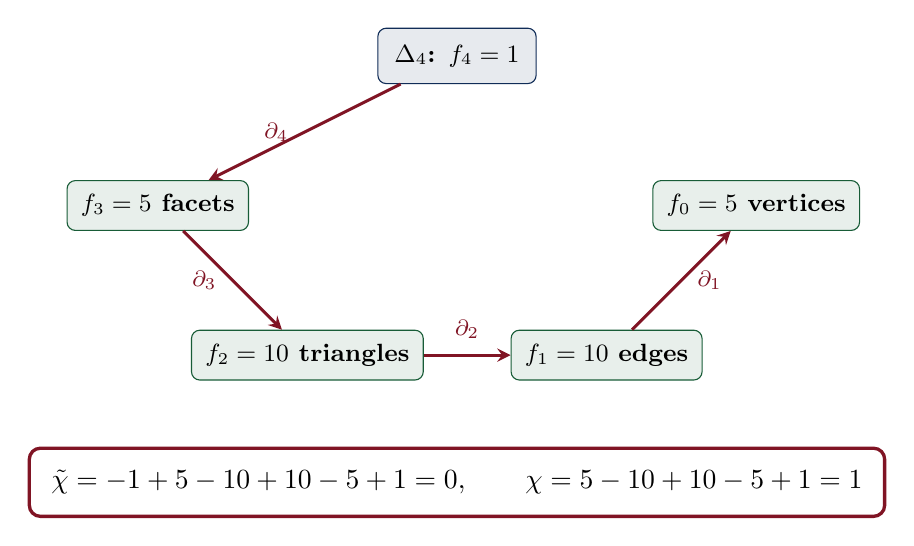
\begin{tikzpicture}[scale=0.95, >=stealth]
    \node[draw=navyblue, fill=navyblue!10, rounded corners=3pt, inner sep=6pt, font=\small\bfseries] (d4) at (0, 2.5) {$\Delta_4$: $f_4 = 1$};
    \node[draw=forestgreen, fill=forestgreen!10, rounded corners=3pt, inner sep=5pt, font=\small\bfseries] (d3) at (-4, 0.5) {$f_3 = 5$ facets};
    \node[draw=forestgreen, fill=forestgreen!10, rounded corners=3pt, inner sep=5pt, font=\small\bfseries] (d2) at (-2.0, -1.5) {$f_2 = 10$ triangles};
    \node[draw=forestgreen, fill=forestgreen!10, rounded corners=3pt, inner sep=5pt, font=\small\bfseries] (d1) at (2.0, -1.5) {$f_1 = 10$ edges};
    \node[draw=forestgreen, fill=forestgreen!10, rounded corners=3pt, inner sep=5pt, font=\small\bfseries] (d0) at (4, 0.5) {$f_0 = 5$ vertices};

    \draw[->, line width=1.1pt, burgundy] (d4) -- (d3) node[midway, left=2pt, font=\footnotesize] {$\partial_4$};
    \draw[->, line width=1.1pt, burgundy] (d3) -- (d2) node[midway, left=2pt, font=\footnotesize] {$\partial_3$};
    \draw[->, line width=1.1pt, burgundy] (d2) -- (d1) node[midway, above=2pt, font=\footnotesize] {$\partial_2$};
    \draw[->, line width=1.1pt, burgundy] (d1) -- (d0) node[midway, right=2pt, font=\footnotesize] {$\partial_1$};

    \node[draw=burgundy, fill=white, line width=1.2pt, rounded corners=4pt, inner sep=8pt] at (0, -3.2) {
        $\displaystyle \tilde\chi = -1 + 5 - 10 + 10 - 5 + 1 = 0, \qquad \chi = 5 - 10 + 10 - 5 + 1 = 1$
    };
\end{tikzpicture}
\caption{Face numbers of the 4-simplex and the boundary maps of its simplicial chain complex. The alternating sums are the Euler characteristic $\chi$ and the reduced Euler characteristic $\tilde\chi$ (empty face included). They are combinatorial identities; see Remark~\ref{rem:cc_counting}.}
\label{fig:cc_cancellation}
\end{figure}

\subsection{An exponential ansatz for the residual density}
Let $\mathcal{E}_\infty = \ln 2 - \frac12 = 0.19315$ be the coefficient of the entropy defect of the continuous Pascal simplex, $\lim_{x\to\infty}(x^2\ln 2 - \mathcal{E}(x))/x^2$ \cite[Ch.~6]{silvafilho2026book}. Consider the ansatz
\begin{equation}\label{eq:cc_ansatz}
    \rho = M_P^4 \exp\left( - \frac{2\pi}{\alpha\, \mathcal{E}_\infty} \right),
\end{equation}
in which the exponent is dimensionless and $\rho$ has dimension $\text{GeV}^4$. The observed dark-energy density, from $\rho_\Lambda = \Omega_\Lambda \cdot 3H_0^2/(8\pi G_N)$ with $H_0 = 67.36\text{ km\,s}^{-1}\text{Mpc}^{-1}$ and $\Omega_\Lambda = 0.6847$ \cite{planck2018}, is
\begin{equation}
    \rho_\Lambda = 2.52 \times 10^{-47}\text{ GeV}^4 = (2.239\text{ meV})^4 = 5.8 \times 10^{-30}\text{ g\,cm}^{-3}.
\end{equation}

\begin{remark}[Status of \eqref{eq:cc_ansatz}]\label{rem:cc_fit}
With $M_P = G_N^{-1/2} = 1.2209\times10^{19}\text{ GeV}$, \eqref{eq:cc_ansatz} equals $\rho_\Lambda$ for $\alpha = 0.1149$; with the reduced Planck mass $M_P/\sqrt{8\pi}$ it requires $\alpha = 0.1176$. The sensitivity is extreme: $\mathrm{d}\ln\rho/\mathrm{d}\alpha = 2\pi/(\alpha^2\mathcal{E}_\infty) \approx 2.5\times10^{3}$, so a $1\%$ change of $\alpha$ changes $\rho$ by a factor $17$. For example, $\alpha = 0.115$ gives $\rho^{1/4} = 2.37\text{ meV}$. The combination $\alpha = \alpha_{\GUT}/(\operatorname{Vol}(\Delta_4)\, C)$ with $\alpha_{\GUT} = 1/24.5$, $\operatorname{Vol}(\Delta_4) = \sqrt5/96$ (unit edge length) and $C = 15.1$ gives $\alpha = 0.11605$, hence $\rho^{1/4} = 4.49\text{ meV}$ and $\rho = 16\,\rho_\Lambda$; the value that reproduces $\rho_\Lambda$ is $C = 15.25$. The constant $C$ has no independent definition, so \eqref{eq:cc_ansatz} is a one-parameter fit to one observable. What it shows is only that an exponent of order $2\pi/(0.1 \times 0.2) \approx 300$ gives a suppression of order $e^{-280} \approx 10^{-122}$. The fractional trace operators of \cite[Ch.~5]{silvafilho2026book} do not produce \eqref{eq:cc_ansatz}.
\end{remark}

% ==============================================================================
\section{Observables, Classification, and Parameter Count}\label{sec:count}
% ==============================================================================

Table~\ref{tab:observables} lists every observable compared in this paper, the formula used, its class (Section~1), and the result with PDG~2024 inputs. Table~\ref{tab:count} counts the continuous inputs.

\begin{table}[htbp]
\centering
\small
\begin{tabular}{@{}L{2.6cm}L{3.6cm}L{2.5cm}L{2.3cm}L{3.2cm}@{}}
\toprule
\textbf{Observable} & \textbf{Formula} & \textbf{Class} & \textbf{Measured} & \textbf{Model; pull} \\
\midrule
$N_g$ & choice of $\Delta_2$ & input & $3$ & $3$ by construction \\
$m_\tau$ [MeV] & $Q_l = 2/3$ with $m_e, m_\mu$ & known relation; prediction & $1776.93 \pm 0.09$ & $1776.97$; $+0.4\sigma$ \\
$Q_{cbt}$ & $\frac23(1 + \alpha_s/\sqrt3)$ & fit (form chosen) & $0.65$--$0.72$ (scheme) & $0.712$; no weight \\
$|V_{us}|$ & $\sqrt{m_d/m_s}$ & known relation & $0.22431(85)$ & $0.2242(19)$; $0.0\sigma$ \\
$\delta_{\mathrm{CKM}}$ [rad] & $\pi/3 + \alpha_s/\sqrt3$ & ansatz & $1.147(26)$ & $1.115$; $-1.2\sigma$ \\
$J_{\mathrm{CP}}$ [$10^{-5}$] & standard param.\ with fitted $s_{23}, s_{13}$ & consistency check & $3.12^{+0.13}_{-0.12}$ & $3.09$; $-0.3\sigma$ \\
$m_3$ [meV] & $v^2/M$ & fit ($M$) & $50.3$ & $30.3$ for $M = 2\times10^{15}$ GeV \\
$\sin^2\theta_{12}$ & $1/3$ & known ansatz & $0.307(13)$ & $0.333$; $+2.0\sigma$ \\
$\sin^2\theta_{23}$ & $1/2$ & known ansatz & $0.558^{+0.015}_{-0.021}$ & $0.500$; $-2.8\sigma$ \\
$\sin\theta_{13}$ & $\sin\theta_C/\sqrt2$ & known ansatz & $0.1480(24)$ & $0.159$--$0.160$; $+4.5$ to $+5.1\sigma$ \\
$\rho_\Lambda^{1/4}$ [meV] & \eqref{eq:cc_ansatz} & fit ($\alpha$ or $C$) & $2.239$ & any value, by tuning $\alpha$ \\
\bottomrule
\end{tabular}
\caption{Observables compared in this paper. Measured values: PDG~2024 \cite{pdg2024} and Planck~2018 \cite{planck2018}. Pulls use the experimental uncertainty only, except for $|V_{us}|$, where the uncertainty of $m_d/m_s$ is included.}
\label{tab:observables}
\end{table}

\begin{table}[htbp]
\centering
\small
\begin{tabular}{@{}L{5.2cm}L{9.8cm}@{}}
\toprule
\textbf{Category} & \textbf{Items} \\
\midrule
Free model parameters (4) & $a$, $\delta$ of the lepton circulant; the scale $M$; the coupling $\alpha$ in \eqref{eq:cc_ansatz} (equivalently $C$) \\
Measured inputs (5) & $\alpha_s(M_Z)$; $m_d/m_s$; $s_{23}$; $s_{13}$; $M_P$ (with a choice of convention) \\
Discrete choices ($\ge 8$) & $b/a = 1/\sqrt2$; the factor $1/\sqrt3$ (used twice); the offset $\pi/3$; the values $1/3$, $1/2$, $1/\sqrt2$ in the PMNS ansatz; the numerator $2\pi$ and the constant $\mathcal{E}_\infty$ in \eqref{eq:cc_ansatz}; the choice of the triplet $(c,b,t)$ \\
\midrule
Observables compared (12) & $m_e$, $m_\mu$, $m_\tau$, $Q_{cbt}$, $|V_{us}|$, $\delta_{\mathrm{CKM}}$, $J_{\mathrm{CP}}$, $m_3$, $\theta_{12}$, $\theta_{23}$, $\theta_{13}$, $\rho_\Lambda$ \\
Used to fix parameters (4) & $m_e$, $m_\mu$, $m_3$, $\rho_\Lambda$ \\
Not independent of inputs (2) & $J_{\mathrm{CP}}$ (proportional to the inputs $s_{23}s_{13}$); $Q_{cbt}$ (scheme spread larger than the claimed agreement) \\
Remaining tests (6) & $m_\tau$ and $|V_{us}|$ pass, and both are relations published in 1982--83 and 1968; $\delta_{\mathrm{CKM}}$ at $1.2\sigma$; $\theta_{12}$ at $2.0\sigma$; $\theta_{23}$ at $2.8\sigma$; $\theta_{13}$ at $4.5$--$5.1\sigma$ \\
\bottomrule
\end{tabular}
\caption{Parameter count. Nine continuous inputs and at least eight discrete choices are set against twelve observables. After the four observables used for calibration and the two that are not independent of the inputs, six tests remain. The two that pass are the known Koide and Gatto--Sartori--Tonin relations. The one new sharp relation, for $\theta_{13}$, is disfavored.}
\label{tab:count}
\end{table}

% ==============================================================================
\section{Conclusion}
% ==============================================================================

The $S_3$ structure of a generation simplex gives a compact language for a few flavor relations. In that language the Koide relation is the statement $b/a = 1/\sqrt2$, i.e.\ a $45^\circ$ angle between the root-mass vector and $(1,1,1)$, and together with $m_e$ and $m_\mu$ it gives $m_\tau$ to $0.4\sigma$. The structure does not select that value, and a circulant ansatz for both quark sectors gives no Cabibbo mixing. The other numbers in this paper are known empirical relations (Gatto--Sartori--Tonin, tri-bimaximal mixing), fits with scheme-dependent or undefined constants ($Q_{cbt}$, the phase ansatz, the neutrino scale, the vacuum-energy exponent), or consistency checks driven by measured inputs ($J_{\mathrm{CP}}$). On the vacuum-energy side, the face-number identities of $\Delta_4$ are exact combinatorics, but no link between them and the zero-point energy is derived, and the exponential ansatz reproduces $\rho_\Lambda$ only after tuning one constant to a few tenths of a percent. Open problems are a derivation of $b/a = 1/\sqrt2$ from a dynamical principle, a mechanism for mixing beyond the circulant ansatz, and a definition of the vacuum-energy weights that would make Remark~\ref{rem:cc_counting} a statement about a quantum field.

% ==============================================================================
\section*{Computational Reproducibility}
% ==============================================================================
No statement in this paper has been formally verified. The Lean~4 files in the author's repository that refer to this material encode the claimed relations as hypotheses of structures with natural-number fields, and restate these hypotheses as theorems; they do not check the mathematics stated here. The mathematical content of the paper consists of the elementary identities of Proposition~\ref{thm:koide_exact}, Remark~\ref{rem:dft} and \eqref{eq:euler}, whose proofs are given or standard. The script \texttt{verify\_fermion\_paper\_numbers.py}, distributed with the paper, recomputes every number from PDG~2024 and Planck~2018 inputs. Each block compares against an independent oracle (a closed form against a root finder, the explicit CKM matrix against the parametrization formula, the critical density from $G_N$ against the PDG expression, two-loop running against published four-loop running masses) and contains a negative control, a mutated formula that must fail the same check.

% ==============================================================================
\section*{Data and Code Availability}
% ==============================================================================
The verification script is distributed with this paper. The author's repository is at \url{https://github.com/reinaldomsilvafilho-netizen/quantum-gravity-lean4}, and the monograph \cite{silvafilho2026book} is archived on Zenodo under \href{https://doi.org/10.5281/zenodo.22290043}{doi:10.5281/zenodo.22290043}.

% ==============================================================================
\begin{thebibliography}{99}
\raggedright

\bibitem{cabibbo1963unitary}
N.~Cabibbo,
\emph{Unitary symmetry and leptonic decays},
Phys. Rev. Lett. \textbf{10} (1963), no.~12, 531--533.
\href{https://doi.org/10.1103/PhysRevLett.10.531}{doi:10.1103/PhysRevLett.10.531}.

\bibitem{gatto1968relation}
R.~Gatto, G.~Sartori, and M.~Tonin,
\emph{Weak self-masses, Cabibbo angle, and broken $\mathrm{SU}(2) \times \mathrm{SU}(2)$},
Phys. Lett. B \textbf{28} (1968), no.~2, 128--130.
\href{https://doi.org/10.1016/0370-2693(68)90150-0}{doi:10.1016/0370-2693(68)90150-0}.

\bibitem{chamseddine2007gravity}
A.~H. Chamseddine, A.~Connes, and M.~Marcolli,
\emph{Gravity and the standard model with neutrino mixing},
Adv. Theor. Math. Phys. \textbf{11} (2007), no.~6, 991--1089.
\href{https://doi.org/10.4310/ATMP.2007.v11.n6.a3}{doi:10.4310/ATMP.2007.v11.n6.a3}.

\bibitem{harrison2002tribimaximal}
P.~F. Harrison, D.~H. Perkins, and W.~G. Scott,
\emph{Tri-bimaximal mixing and the neutrino oscillation data},
Phys. Lett. B \textbf{530} (2002), 167--173.
\href{https://doi.org/10.1016/S0370-2693(02)01336-9}{doi:10.1016/S0370-2693(02)01336-9}.

\bibitem{huang2021precise}
G.-Y. Huang and S.~Zhou,
\emph{Precise values of running quark and lepton masses in the standard model},
Phys. Rev. D \textbf{103} (2021), 016010.
\href{https://doi.org/10.1103/PhysRevD.103.016010}{doi:10.1103/PhysRevD.103.016010}.

\bibitem{jarlskog1985commutator}
C.~Jarlskog,
\emph{Commutator of the quark mass matrices in the standard electroweak model and a measure of maximal CP nonconservation},
Phys. Rev. Lett. \textbf{55} (1985), no.~10, 1039--1042.
\href{https://doi.org/10.1103/PhysRevLett.55.1039}{doi:10.1103/PhysRevLett.55.1039}.

\bibitem{kobayashi1973cp}
M.~Kobayashi and T.~Maskawa,
\emph{CP-violation in the renormalizable theory of weak interaction},
Prog. Theor. Phys. \textbf{49} (1973), no.~2, 652--657.
\href{https://doi.org/10.1143/PTP.49.652}{doi:10.1143/PTP.49.652}.

\bibitem{king2012tbc}
S.~F. King,
\emph{Tri-bimaximal-Cabibbo mixing},
Phys. Lett. B \textbf{718} (2012), 136--142.
\href{https://doi.org/10.1016/j.physletb.2012.10.028}{doi:10.1016/j.physletb.2012.10.028}.

\bibitem{koide1982}
Y.~Koide,
\emph{Fermion-boson two-body model of quarks and leptons and Cabibbo mixing},
Lett. Nuovo Cimento \textbf{34} (1982), 201--205.
\href{https://doi.org/10.1007/BF02817096}{doi:10.1007/BF02817096}.

\bibitem{koide1983fermion}
Y.~Koide,
\emph{A fermion-boson composite model of quarks and leptons},
Phys. Lett. B \textbf{120} (1983), no.~1-3, 161--165.
\href{https://doi.org/10.1016/0370-2693(83)90644-5}{doi:10.1016/0370-2693(83)90644-5}.

\bibitem{maki1962remarks}
Z.~Maki, M.~Nakagawa, and S.~Sakata,
\emph{Remarks on the unified model of elementary particles},
Prog. Theor. Phys. \textbf{28} (1962), no.~5, 870--880.
\href{https://doi.org/10.1143/PTP.28.870}{doi:10.1143/PTP.28.870}.

\bibitem{pdg2024}
S.~Navas et~al. (Particle Data Group),
\emph{Review of Particle Physics},
Phys. Rev. D \textbf{110} (2024), no.~3, 030001.
\href{https://doi.org/10.1103/PhysRevD.110.030001}{doi:10.1103/PhysRevD.110.030001}.

\bibitem{planck2018}
N.~Aghanim et~al. (Planck Collaboration),
\emph{Planck 2018 results. VI. Cosmological parameters},
Astron. Astrophys. \textbf{641} (2020), A6.
\href{https://doi.org/10.1051/0004-6361/201833910}{doi:10.1051/0004-6361/201833910}.

\bibitem{silvafilho2026book}
R.~M. Silva-Filho,
\emph{Geometry, Tensors, and Quantum Gravity},
monograph, Zenodo (2026).
\href{https://doi.org/10.5281/zenodo.22290043}{doi:10.5281/zenodo.22290043}.

\bibitem{weinberg1979baryon}
S.~Weinberg,
\emph{Baryon- and lepton-nonconserving processes},
Phys. Rev. Lett. \textbf{43} (1979), no.~21, 1566--1570.
\href{https://doi.org/10.1103/PhysRevLett.43.1566}{doi:10.1103/PhysRevLett.43.1566}.

\bibitem{weinberg1967model}
S.~Weinberg,
\emph{A model of leptons},
Phys. Rev. Lett. \textbf{19} (1967), no.~21, 1264--1266.
\href{https://doi.org/10.1103/PhysRevLett.19.1264}{doi:10.1103/PhysRevLett.19.1264}.

\bibitem{weinberg1989cosmological}
S.~Weinberg,
\emph{The cosmological constant problem},
Rev. Mod. Phys. \textbf{61} (1989), no.~1, 1--23.
\href{https://doi.org/10.1103/RevModPhys.61.1}{doi:10.1103/RevModPhys.61.1}.

\end{thebibliography}

\end{document}
